\begin{figure}[H]
\centering
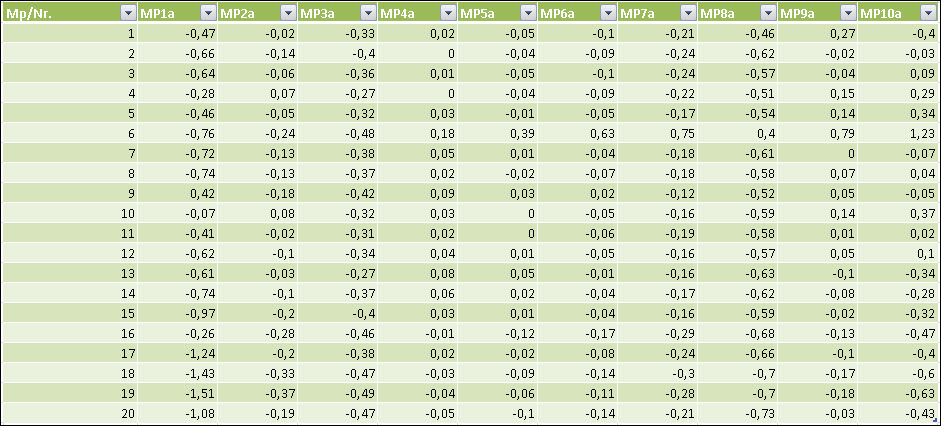
\includegraphics[width=.8\textwidth]{F13Bieg}
\caption{Messwerte F13 Streckbiegen. Erste Versuchsreihe.}
\label{F13Bieg}
\end{figure}
\begin{figure}[H]
\centering
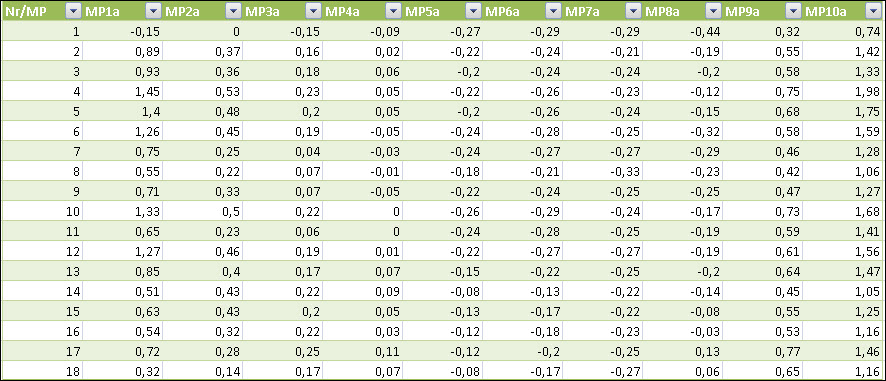
\includegraphics[width=.8\textwidth]{FxxBieg}
\caption{Messwerte Fxx Streckbiegen. Erste Versuchsreihe.}
\label{FxxBieg}
\end{figure}
\begin{figure}[H]
\centering
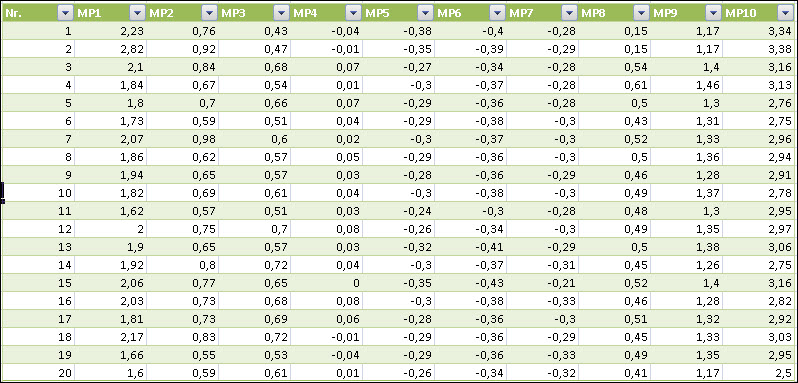
\includegraphics[width=.8\textwidth]{F17Bieg}
\caption{Messwerte F17 Streckbiegen. Erste Versuchsreihe.}
\label{F17Bieg}
\end{figure}
\begin{figure}[H]
\centering
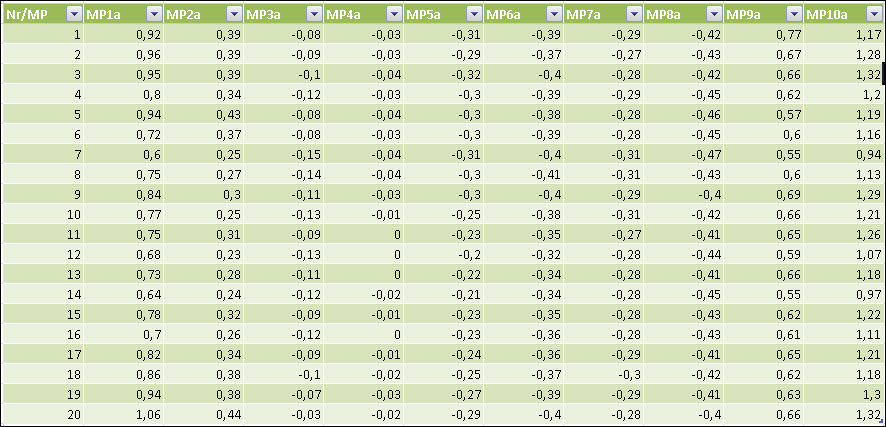
\includegraphics[width=.8\textwidth]{nFxxBieg}
\caption{Messwerte nFxx Streckbiegen. Zweite Versuchsreihe.}
\label{nFxxBieg}
\end{figure}
\begin{figure}[H]
\centering
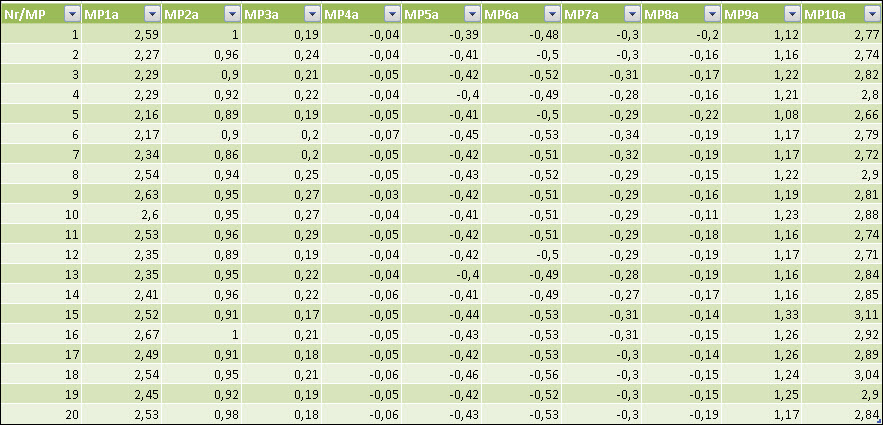
\includegraphics[width=.8\textwidth]{nF17Bieg}
\caption{Messwerte nF17 Streckbiegen. Zweite Versuchsreihe.}
\label{nF17Bieg}
\end{figure}
\begin{figure}[H]
\centering
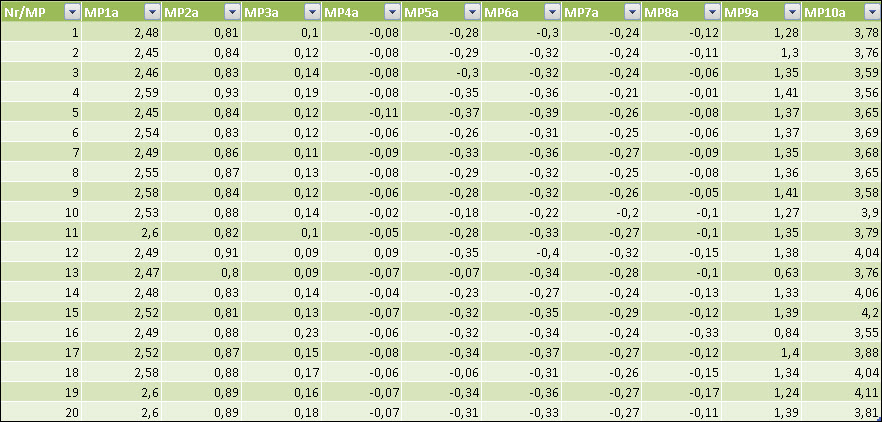
\includegraphics[width=.8\textwidth]{F18Bieg}
\caption{Messwerte F18 Streckbiegen. Zweite Versuchsreihe.}
\label{F18Bieg}
\end{figure}
\begin{figure}[H]
\centering
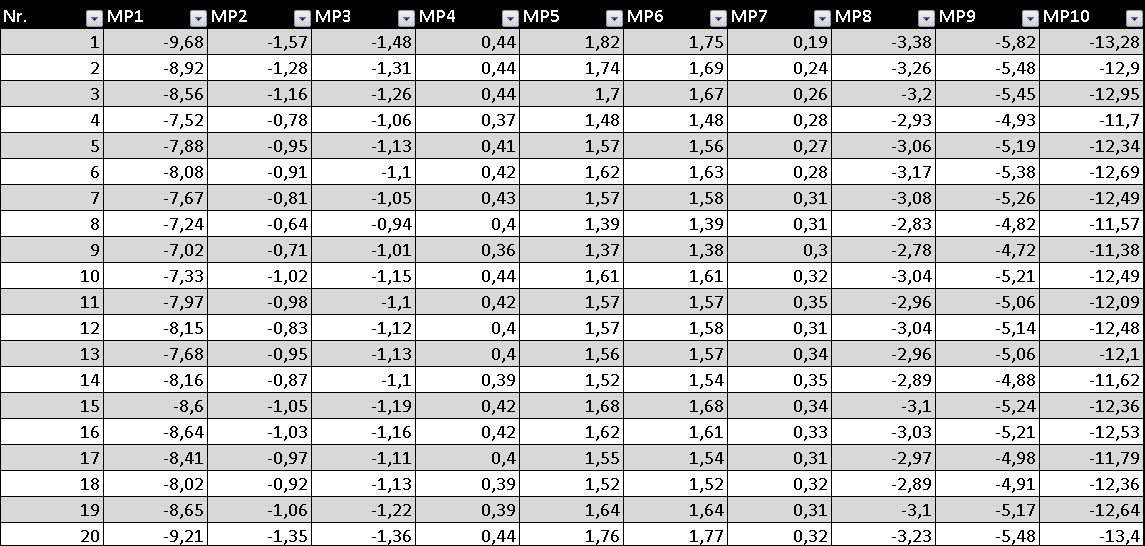
\includegraphics[width=.8\textwidth]{F19Bieg}
\caption{Messwerte F19 Streckbiegen. Zweite Versuchsreihe.}
\label{F19Bieg}
\end{figure}
\begin{figure}[H]
\centering
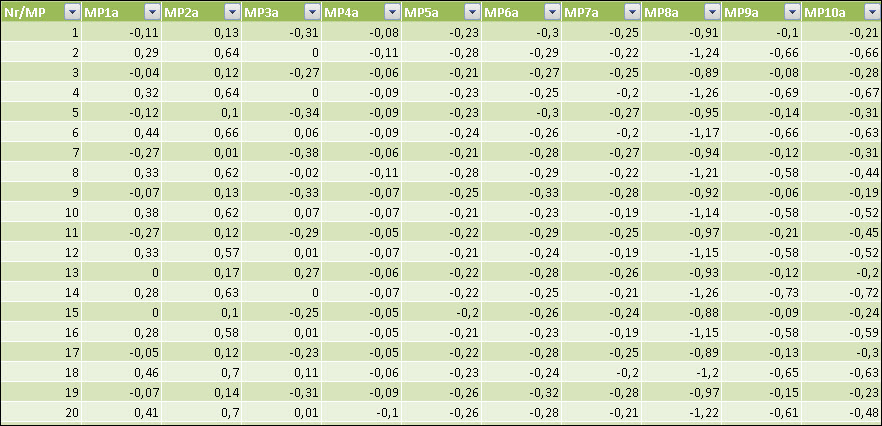
\includegraphics[width=.8\textwidth]{F13fraes}
\caption{Messwerte F13 Fräsen.}
\label{F13fraes}
\end{figure}
\begin{figure}[H]
\centering
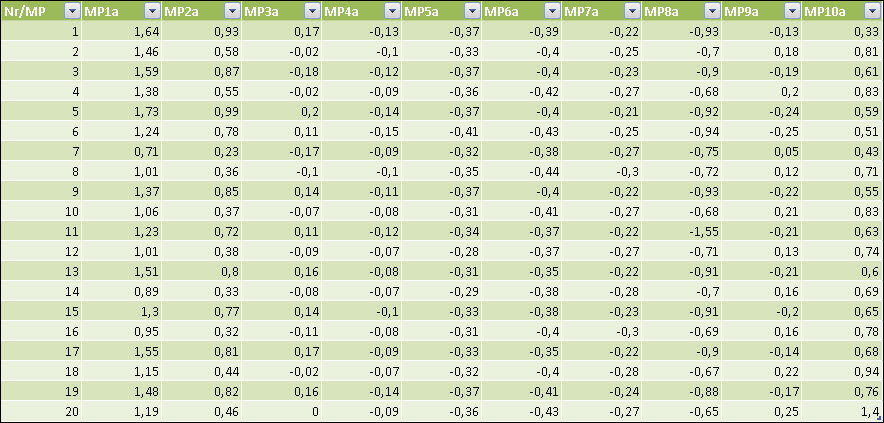
\includegraphics[width=.8\textwidth]{Fxxfraes}
\caption{Messwerte Fxx Fräsen.}
\label{Fxxfraes}
\end{figure}
\begin{figure}[H]
\centering
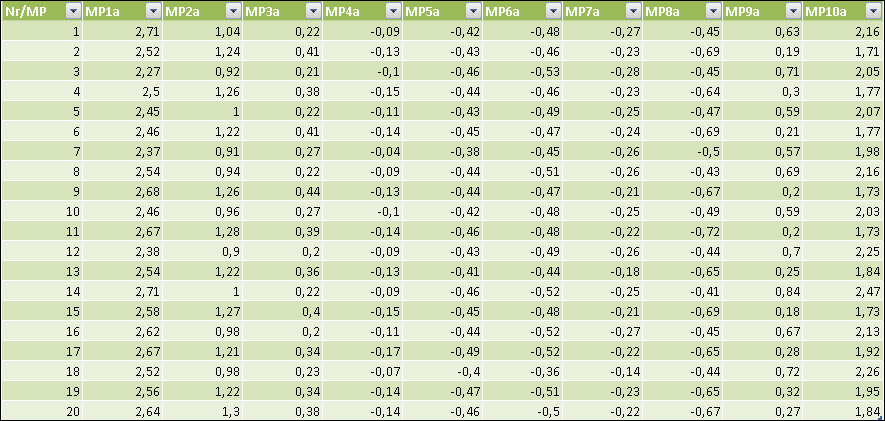
\includegraphics[width=.8\textwidth]{F17fraes}
\caption{Messwerte F17 Fräsen.}
\label{F17fraes}
\end{figure}
\begin{figure}[H]
\centering
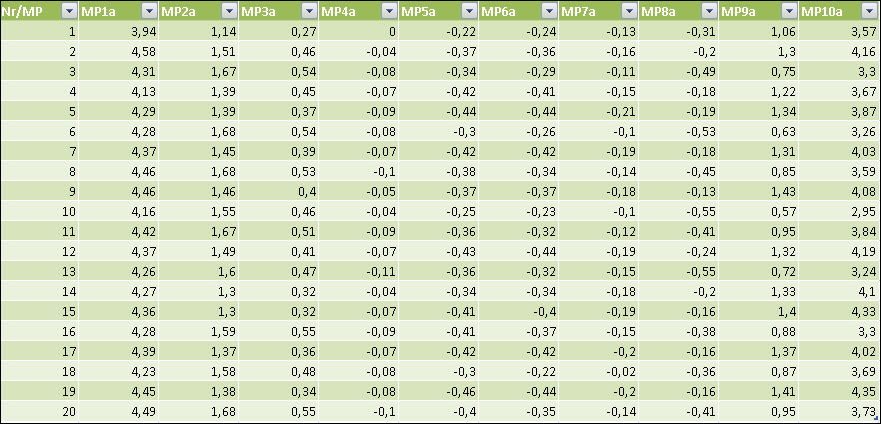
\includegraphics[width=.8\textwidth]{F18fraes}
\caption{Messwerte F18 Fräsen.}
\label{F18 fraes}
\end{figure}
\begin{figure}[H]
\centering
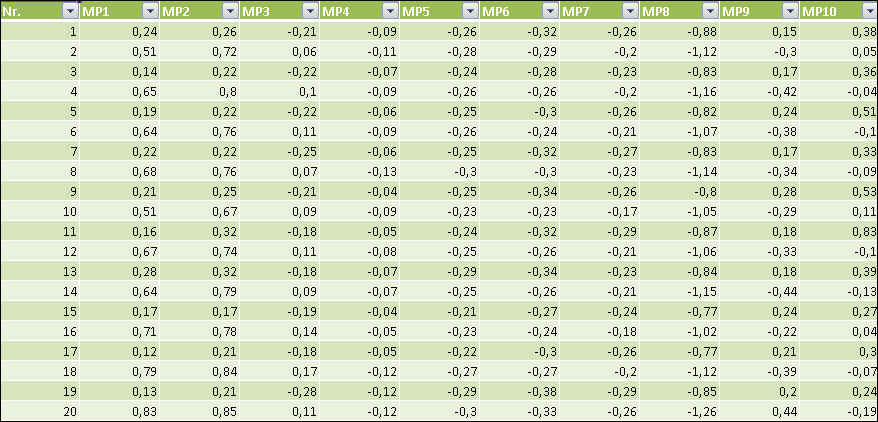
\includegraphics[width=.8\textwidth]{F13polier}
\caption{Messwerte F13 Polieren.}
\label{F13polier}
\end{figure}
\begin{figure}[H]
\centering
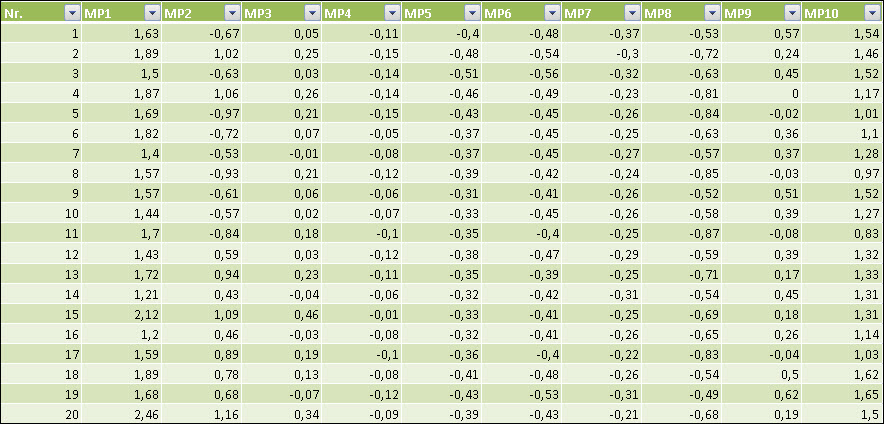
\includegraphics[width=.8\textwidth]{Fxxpolier}
\caption{Messwerte Fxx Polieren.}
\label{Fxxpolier}
\end{figure}
\begin{figure}[H]
\centering
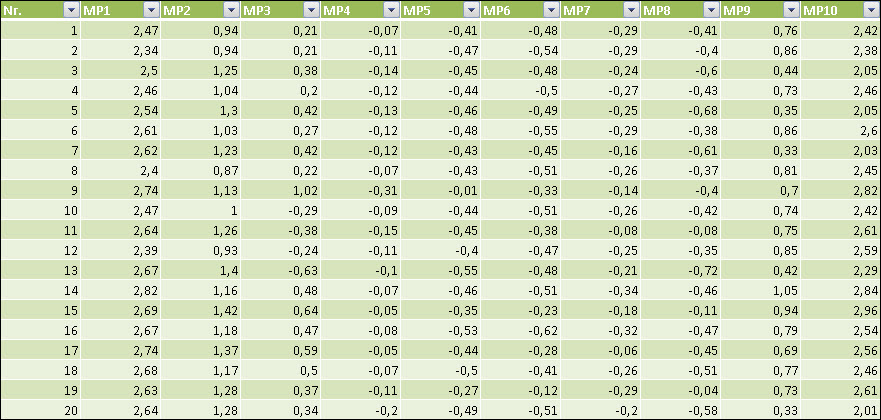
\includegraphics[width=.8\textwidth]{F17polier}
\caption{Messwerte F17 Polieren.}
\label{F17polier}
\end{figure}
\begin{figure}[H]
\centering
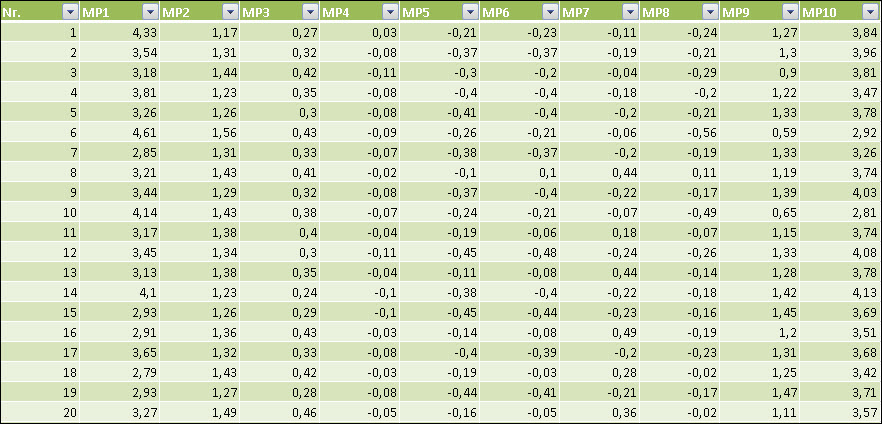
\includegraphics[width=.8\textwidth]{F18polier}
\caption{Messwerte F18 Polieren}
\label{F18polier}
\end{figure}
\begin{figure}[H]
\centering
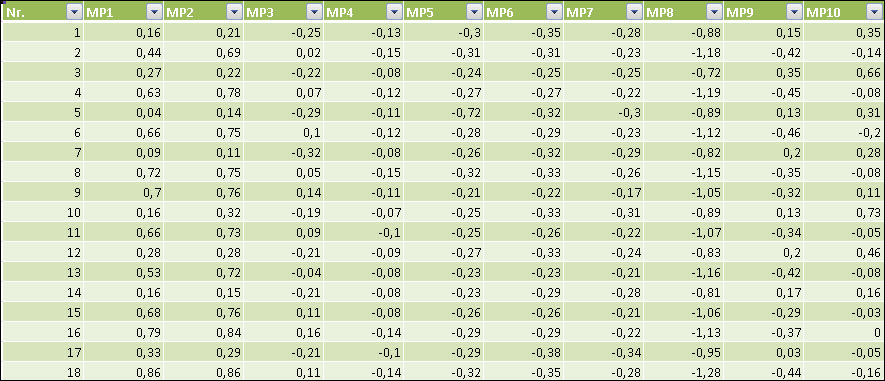
\includegraphics[width=.8\textwidth]{F13elox}
\caption{Messwerte F13 Eloxieren.}
\label{F13elox}
\end{figure}
\begin{figure}[H]
\centering
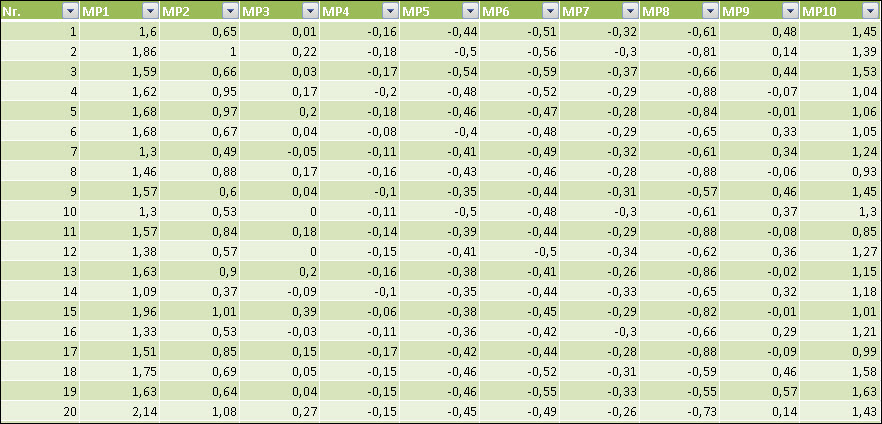
\includegraphics[width=.8\textwidth]{Fxxelox}
\caption{Messwerte Fxx Eloxieren.}
\label{Fxxelox}
\end{figure}
\begin{figure}[H]
\centering
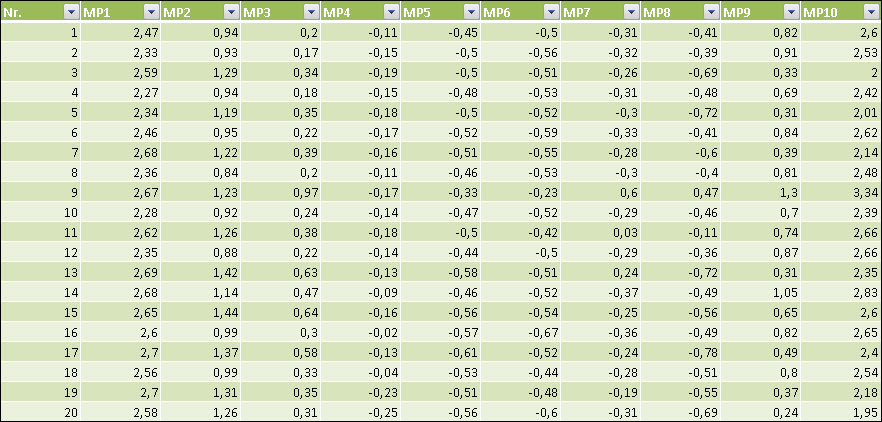
\includegraphics[width=.8\textwidth]{F17elox}
\caption{Messwerte F17 Eloxieren.}
\label{F17elox}
\end{figure}
\begin{figure}[H]
\centering
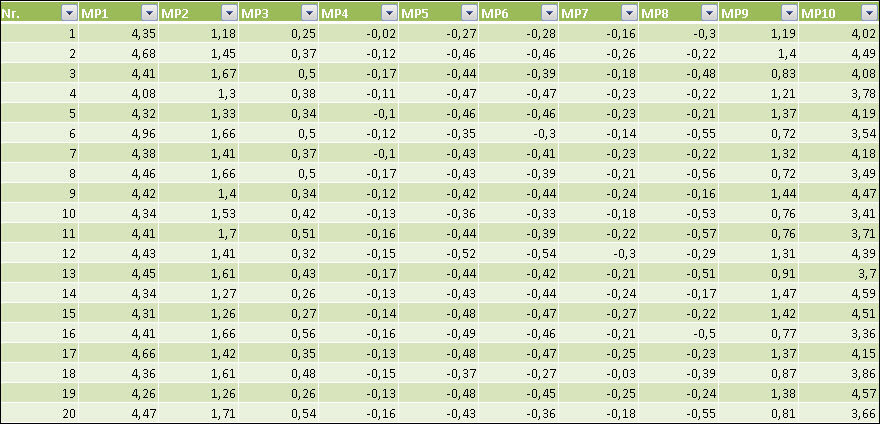
\includegraphics[width=.8\textwidth]{F18elox}
\caption{Messwerte F18 Eloxieren.}
\label{F18elox}
\end{figure}
\begin{figure}[H]
\centering
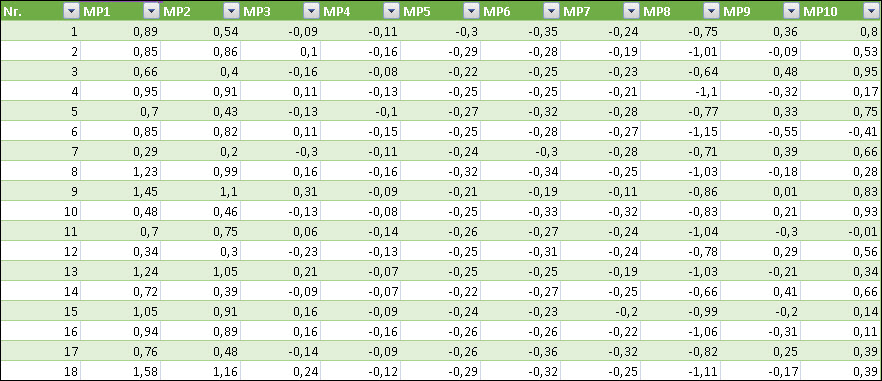
\includegraphics[width=.8\textwidth]{F13durapro}
\caption{Messwerte F13 DURApro.}
\label{F13durapro}
\end{figure}
\begin{figure}[H]
\centering
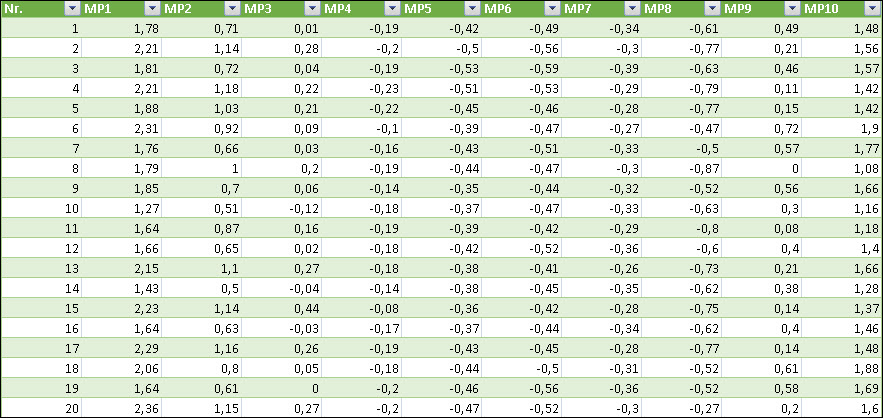
\includegraphics[width=.8\textwidth]{Fxxdurapro}
\caption{Messwerte Fxx DURApro.}
\label{Fxxdurapro}
\end{figure}
\begin{figure}[H]
\centering
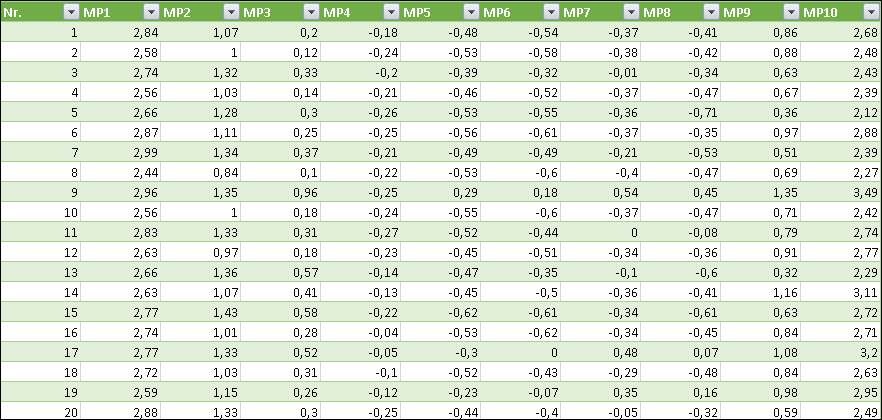
\includegraphics[width=.8\textwidth]{F17durapro}
\caption{Messwerte F17 DURApro.}
\label{F17durapro}
\end{figure}
\begin{figure}[H]
\centering
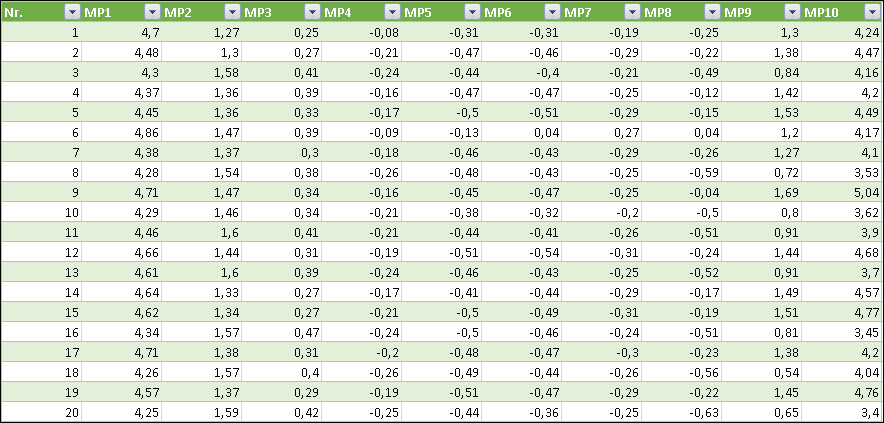
\includegraphics[width=.8\textwidth]{F18durapro}
\caption{Messwerte F18 DURApro}
\label{F18durapro}
\end{figure}



















